\documentclass[submission,copyright,creativecommons]{eptcs}

\providecommand{\event}{PLACES 2019}

\usepackage[utf8]{inputenc}
\usepackage[T1]{fontenc}
\usepackage{color}
\usepackage{listings}
\usepackage{tikz}
\usepackage{wrapfig}
\usepackage{amsmath,amssymb,stmaryrd}
\usepackage[portuguese]{babel}
\usepackage[utf8]{inputenc}  % for proper diacritics
\usepackage[T1]{fontenc}
\usepackage {listings}
\usepackage{tikz}
% \usepackage{xcolor}
% Links
\usepackage{hyperref}

\usepackage{amsmath,amssymb}
%\usepackage{stmaryrd}
\usepackage{listings,color}
\usepackage{alltt}
\usepackage{flushend}



%\usepackage[T1]{fontenc}

% \lstdefinestyle{Go}{	
% 	keywordstyle=[1]\bfseries,
% 	basicstyle=\footnotesize\ttfamily,	
% 	numberstyle=\tiny,
% 	numbersep=5pt,
% 	breaklines=true,
% 	%prebreak=\raisebox{0ex}[0ex2][0ex]{\ensuremath{\hookleftarrow}},
% 	showstringspaces=false,
% 	upquote=true,
% 	tabsize=3,
% 	frame=tb,
% 	morekeywords={go,make,chan,int,import,main,func,for,select,case,string},
%       }

\lstdefinelanguage{Golang}%
  {morekeywords=[1]{package,import,func,type,struct,return,defer,panic,%
     recover,select,var,const,iota,},%
   morekeywords=[2]{string,uint,uint8,uint16,uint32,uint64,int,int8,int16,%
     int32,int64,bool,float32,float64,complex64,complex128,byte,rune,uintptr,%
     error,interface},%
   morekeywords=[3]{map,slice,make,new,nil,len,cap,copy,close,true,false,%
     delete,append,real,imag,complex,chan,},%
   morekeywords=[4]{for,break,continue,range,goto,switch,case,fallthrough,if,%
     else,default,},%
   morekeywords=[5]{Println,Printf,Error,Print,},%
   sensitive=true,%
   morecomment=[l]{//},%
   morecomment=[s]{/*}{*/},%
   morestring=[b]',%
   morestring=[b]",%
   morestring=[s]{`}{`},%
}

      
\lstdefinelanguage{SePi}%
  {morekeywords=[1]{type,integer,string,boolean,new, select, assume, assert},%
   sensitive=true,%
   morecomment=[l]{//},%
   morecomment=[s]{/*}{*/},%
   morestring=[b]',%
   morestring=[b]",%
   morestring=[s]{`}{`},%
 }

\lstdefinelanguage{CFST}%
{
  morekeywords=[1]{Int, Char, Bool, Skip, forall, rec, let, in, if, then, else, new, send, receive,
    select, fork, case, of, data, match, with},%  
  sensitive=true,%
  literate={->}{{$\rightarrow$}}1,%
   breaklines=true,
   morecomment=[l]{--},%
   morecomment=[s]{{-}{-}},%
   morestring=[b]',%
   morestring=[b]",%
   morestring=[s]{`}{`},%
 }

 

% notes
\newcommand{\todo}[1]{[{\color{blue}\textbf{#1}}]}

% Keywords
\newcommand{\keyword}[1]{\mathsf{#1}}

% Prekinds

\newcommand\prekind{\upsilon}

\newcommand{\stypes}{\mathcal S}
\newcommand\kinds{\stypes}

\newcommand{\types}{\mathcal T}
\newcommand\kindt{\types}

\newcommand\kindsch{\mathcal C}

% Multiplicity
\newcommand\Un{\ensuremath{\mathbf{u}}} % \infty
\newcommand\Lin{\ensuremath{\mathbf{l}}} % 1 

% Kinds
\newcommand\kind{\kappa}

% Grammars
\newcommand{\grmeq}{\; ::= \;}
\newcommand{\grmor}{\;\mid\;}

% type constructors
\newcommand\tcBase{B}
\newcommand\tcLolli\multimap
\newcommand\tcFun\to
\newcommand\tcBang{\mathop!}

% Keywords for types
\newcommand\kRec{\keyword{rec}}


% Types
\newcommand{\tskip}{\keyword{Skip}}
\newcommand\tSemi[2]{#1;#2}
\newcommand\tOut[1]{\tcBang#1}
\newcommand\tIn[1]{?#1}
\newcommand\tIChoice[1]{\oplus#1}
\newcommand\tEChoice[1]{\&#1}
\newcommand\tUnFun[2]{#1\tcFun#2}
\newcommand\tLinFun[2]{#1\tcLolli#2}
\newcommand\tPair[2]{#1\otimes#2}
\newcommand\tDatatype[1]{{[#1]}}
\newcommand\tRec[2]{\mu\,#1\,.\,#2}
\newcommand\tForall[2]{\forall\,#1\,.\,#2}

\newcommand\tRecK[2]{\kRec\,#1\,.\,#2}
% Environments
% \newcommand\emptyEnv{\cdot}
\newcommand\emptyEnv{\varepsilon}
\newcommand\kindEnv{\Delta}
\newcommand\varEnv{\Gamma}

% Language
% Expressions
% Language Types
\newcommand{\unite}{\keyword{Unit}}
\newcommand{\inte}{\keyword{Int}}
\newcommand{\chare}{\keyword{Char}}
\newcommand{\boole}{\keyword{Bool}}

% Variables
\newcommand\vare[1]{#1}
\newcommand\unlete[3]{\keyword{let} \; #1 = #2 \; \keyword{in} \; #3} 

% Applications
\newcommand\appe[2]{#1#2}
\newcommand\tappe[2]{#1[#2]}

% Conditional
\newcommand\conditionale[3]{\keyword{if}\;#1\;\keyword{then}\;#2\;\keyword{else} \; #3}

% Pairs
\newcommand\paire[2]{(#1,#2)}
\newcommand\binlete[4]{\keyword{let}\;#1, #2 = #3\;\keyword{in}\;#4}

% Session Types
\newcommand\newe[1]{\keyword{new}\;#1}
\newcommand\sende[2]{\keyword{send}\;#1\; #2}
\newcommand\recve[1]{\keyword{receive}\;#1}
\newcommand\selecte[1]{\keyword{select}\;#1}
\newcommand\matche[2]{\keyword{match}\;#1\;\keyword{with}\;#2}

% Fork
\newcommand\forke[1]{\keyword{fork}\;#1}

% Datatypes
\newcommand{\ctrcte}{C}
\newcommand\casee[2]{\keyword{case}\;#1\;\keyword{of}\;#2}

% Goal
\newcommand\Alg{\vdash_{a}}

% Equivalent
\newcommand\Equiv[2]{#1\,\thicksim\,#2}


%%% Local Variables:
%%% mode: latex
%%% TeX-master: "cfst-inforum18"
%%% End:
      

\title{FreeST: context-free session types in a functional language}
\author{
  Bernardo Almeida
  \and
  Andreia Mordido
  \and
  Vasco T. Vasconcelos
  \institute{LASIGE, Faculdade de Ciências, Universidade de Lisboa, Portugal}
}
\def\titlerunning{\freest}
\def\authorrunning{Almeida, Mordido \& Vasconcelos}

\begin{document}
\maketitle
\begin{abstract}
  We present an algorithm to decide the equivalence of context-free
  session types, practical to the point of being incorporated in a
  compiler. We prove its soundness and completeness. We further study
  its behaviour in practice.

  % mandatory; please add comma-separated list of keywords
  \keywords{Types, Type equivalence, Bisimulation, Algorithm} 
\end{abstract}

  % Session types are paramount to describe the structured interaction
  % of processes via typed communication channels; however, they lack an
  % efficient description for serialization of tree-structured data in a
  % type-safe way.

  % Context-free session types were proposed as an extension of session
  % types able to capture the type-safe serialization of recursive
  % datatypes. For the sake of a practical usage, namely in the
  % definition of new programming languages, there is an urgent need for
  % an algorithm to decide type equivalence. In this work, we propose an
  % algorithm to decide type equivalence on context-free session
  % types. We prove its soundness and completeness, and validate the
  % algorithm on several examples.

%%% Local Variables:
%%% mode: latex
%%% TeX-master: "main"
%%% End:

\section{Session types deserve to be free}

Session types have been long subject to the shackles of tail
recursion~\cite{DBLP:conf/concur/Honda93,DBLP:conf/esop/HondaVK98}. Regular
session-type languages bear the evident advantage of providing for
simple algorithms to check type equivalence and subtyping. Given two
types, a fixed-point construction algorithm such as the one introduced
by Gay and Hole builds, in polynomial time and space, a bisimulation
relating the two types, or decides that no such relation
exists~\cite{DBLP:journals/acta/GayH05}. The scenario darkens when one
decides to let go of tail recursion, for now the fixed-point
construction algorithm does not necessarily terminate.
%
This is one of the main reasons why session types have been confined
to ($\omega$-) regular languages for so many years.

The discipline of conventional (that is, regular) session types
provides guarantees not easily accessible to simpler languages such as
concurrent ML, where channels are unidirectional and transport values
of a fixed size~\cite{DBLP:conf/mcmaster/Reppy93}. Session types, in
turn, provide for the description of richer protocols, epitomised by
the math server~\cite{DBLP:journals/acta/GayH05}, which can be
rendered in the SePi language~\cite{DBLP:conf/sefm/FrancoV13} as
follows:
%
\begin{lstlisting}[morekeywords=end]
MathServer = +{
  Plus: !Int.!Int.?Int.MathServer,
  Eq: !Int.!Int.?Bool.MathServer,
  Done: end
}
\end{lstlisting}

Type \lstinline|MathServer| describes the client side of the protocol,
introducing three choices: \lstinline|Plus|, \lstinline|Eq|, and
\lstinline|Done|. A client that chooses the \lstinline|Plus| choice is
supposed to send two integer values and to receive a further integer
(possibly representing the sum of the former two), after which it goes
back to the beginning. If the same client chooses instead the
\lstinline|Eq| option, it must subsequently send two integer values
and expect a boolean result (possibly describing whether the two
integers are equal), after which it must go back to the beginning.
The \lstinline|Done| option terminates the protocol, as described by
type \lstinline[morekeywords=end]|end|.

The guarantees introduced by session type systems include the
adherence of the code to the protocol and the related absence of
runtime errors, including race
conditions~\cite{DBLP:conf/esop/HondaVK98}. Some systems further
guarantee progress~\cite{DBLP:conf/concur/CairesP10}. All this, under
a rather expressive type language, that of (regular) session types.

There is one further characteristic of session types that attest for
its flexibility: the ability send channels on channels, often called
delegation. This feature provides for the transmission of complex data
on channels in a typeful manner. Suppose we want to stream a tree
%
\begin{lstlisting}
data Tree = Leaf | Node Int Tree Tree
\end{lstlisting}
%
on a channel. One has to choose between a) using multiple channels for
sending the tree or b) incurring on runtime checks to check adherence
to the protocol. In the former scenario, trees are sent on channels of
type
%
\begin{lstlisting}[morekeywords=end]
type TreeChannelR = +{Leaf:end, Node:!Int.!TreeChannelR.!TreeChannelR.end}
\end{lstlisting}
%
and we see that two new channels must be created and exchanged for
each \lstinline|Node| in a tree, so that $2n+1$ channels are needed to
stream an $n$-\lstinline|Node| tree.
%
In the latter case, tree parts are sent on a single stream, but not
necessarily in a ``tree form''. A suitable channel type is
%
\begin{lstlisting}[morekeywords=end]
type TreeParts = +{Leaf: TreeParts, Node: !Int.TreeParts, EOS: end}
\end{lstlisting}
%
where \lstinline|EOS| represents the end of stream. In this case tree
\lstinline|Node 1 (Node 2 Leaf Leaf) Leaf| can be streamed as
\lstinline|Node 1 Node 2 Leaf Leaf Leaf EOS|, when the tree is visited
in a depth-first manner. It should be easy to see that type
\lstinline|TreeParts| allows streaming many different tree parts that
do not add up to a tree, hence the necessary runtime checks to look
over unexpected parts on the stream.

In 2016, Thiemann and Vasconcelos introduced the concept of
context-free session types and proved that type equivalence remains
decidable~\cite{DBLP:conf/icfp/ThiemannV16}.
%
Context-free session types appear as a natural extension of
conventional (regular) session-types. Syntactically, the changes are
minor: rather than dot (\lstinline|.|), the prefix operator, we use
semi-colon (\lstinline|;|), a new binary operator on types. We also
take the chance to replace \lstinline [morekeywords=end]|end| by
\lstinline|Skip| to make it clear that it does not necessarily ``end''
a session type, but else merely introduces a mark that can sometimes
be omitted. In fact \lstinline|Skip| is the identity element of
sequential composition, so that \freest{} enjoys the monoidal axioms:
\lstinline|Skip;T| $\equiv$ \lstinline|T;Skip| $\equiv$ \lstinline|T|,
for all types \lstinline|T|.
%
Using the syntax of \freest, a channel that streams a tree can be
written as follows:
%
\begin{lstlisting}
type TreeChannel = +{Leaf: Skip, Node: !Int;TreeChannel;TreeChannel}
\end{lstlisting}

The language \freest, described in the sequel, provides for the best
of both worlds: stream the tree on a \emph{single} channel,
\emph{without} extraneous runtime checks.

% Related work

There are a few experimental programming languages based on session
types and there are many proposals for encoding session types in
mainstream programming languages. We cannot cover them all in
this short abstract; the interested reader is referred to a 2016
survey on behavioural types in programming
languages~\cite{DBLP:journals/ftpl/AnconaBB0CDGGGH16}.  Here, we briefly
discuss a few prototypical programming languages using session types.

SePi is a programming language based on the pi-calculus whose channels
are governed by regular session types refined with uninterpreted
predicates~\cite{DBLP:conf/sefm/FrancoV13}. The concrete syntax we
choose for \freest{} is heavily influenced by SePi.

SILL is a functional language with session typed concurrency, based on
the Curry-Howard interpretation of intuitionistic linear
logic~\cite{DBLP:conf/concur/CairesP10}, further extended with
recursive types and
processes~\cite{Toninho:phd,DBLP:conf/esop/ToninhoCP13}.
%
C1 is an imperative language~\cite{Pfenning:C1} developed along the
lines of SILL, featuring types that express
sharing~\cite{DBLP:journals/pacmpl/BalzerP17}.
%
All these languages use regular session types. Compared to \freest,
they present stronger properties (including progress), at the expense
of imposing a particular form of programming (derived from the
Curry-Howard interpretation) whereby each process uses zero or more
channels and provides exactly one. At the time of this writing,
\freest{} does not include shared types.

Links~\cite{DBLP:conf/fmco/CooperLWY06} is a functional programming
language for the web, later extended with session types
primitives~\cite{Lindley.Morris_Lightweight.functional.session.types}. Very
much like SILL and C1, the base language is deadlock-free and
terminating. Links also include recursion and shared channels,
foregoing deadlock-freedom.

The only other implementation of context-free session types we are
aware of is that of Padovani~\cite{DBLP:conf/esop/Padovani17}, a
language that admits equivalence, subtyping and, of particular
interest, inference algorithms. It does however require a structural
alignment between the process code and the session types, enforced by
a \emph{resumption} process operator that explicitly breaks a type
$S;T$. The usage of resumptions requires additional annotations
from the programmer---which we would like to avoid in 
\freest---and, beyond that, it does not solve the type equivalence
problem since the monoidal rules proposed by Thiemann and
Vasconcelos cannot be used. Padovani proposes the use of 
\emph{explicit coercions} to fix this limitation, but this
would require a greater effort from the programmer. 
Any additional effort by the programmer is error-prone, hence
we have embedded a type equivalence checker into  
\freest\ so that it does not need to rely on any
additional annotation from the programmer.


%%% Local Variables:
%%% mode: latex
%%% TeX-master: "main"
%%% End:

\section{\freest{} is for programming}
\label{sec:programming}

\freest{} is a basic implementation of the language introduced by
Thiemann and Vasconcelos~\cite{DBLP:conf/icfp/ThiemannV16}. Here we
provide a gentle introduction to the language.
%
We have chosen the concrete syntax to be aligned with that of Haskell,
as much as possible. A \freest{} script is a collection of type
abbreviations, datatype and function (or value) declarations. Function
\lstinline|start| starts it all.

Our first example serializes a tree object on a channel. The datatype
for trees, \lstinline|Tree|, was introduced before.  We also need a
channel capable of transmitting a tree. The type below describes a
variant of the \lstinline|TreeChannel| introduced before that not only
sends a tree, but, for each \lstinline|Node|, also receives back an
integer value.
%
\begin{lstlisting}
type TreeC = +{Leaf: Skip, Node: !Int;TreeC;TreeC;?Int}
\end{lstlisting}

The \lstinline|+| type constructor introduces an internal choice (the
process in possession of the channel end chooses) with two
alternatives, labelled \lstinline|Leaf| and \lstinline|Node|. These
two labels should not be confused with the constructors of 
datatype \lstinline|Tree|. \lstinline|Leaf| states that no further
interaction is possible on the channel (denoted by \lstinline|Skip|);
the \lstinline|Node| branch writes an integer value, followed by two
trees, and terminates by reading an integer value
(\lstinline|!Int;TreeC;TreeC;?Int|).
%
The type declaration introduces an \emph{abbreviation} to a recursive
type \lstinline|rec x. +{Leaf: Skip, Node: !Int;x;x;?Int}|, a type
that is valid in \freest.

The writer process, \lstinline|transform|, writes a tree on a given
channel. The channel is of type \lstinline|TreeC;alpha|, for
\lstinline|alpha| a type variable. It returns a \lstinline|Tree| and
the residual of the input channel, of type \lstinline|alpha|. The type
of \lstinline|transform| is \emph{polymorphic}: different calls to the
function use different values for \lstinline|alpha|.

\begin{lstlisting}
transform: forall alpha => Tree -> TreeC;alpha -> (Tree, alpha)
\end{lstlisting}

For each \lstinline|Node| in the input tree, function
\lstinline|transform| reads an integer from the channel and returns a
tree isomorphic to the input where the integer values in nodes are
read from the channel.
%
The function performs a \lstinline|case| analysis on the
\lstinline|Tree| constructor (either \lstinline|Leaf| or
\lstinline|Node|). In the former case, it \lstinline|select|s the
\lstinline|Leaf| choice and returns a pair composed of the original
tree and the residual of the channel. In the latter case, the function
\lstinline|select|s the \lstinline|Node| choice, then sends the
integer value in the channel, followed by the two subtrees (via
recursive calls). Finally, reads an integer \lstinline|y| from the
channel, assembles a tree with \lstinline|y| at the \lstinline|Node|
and returns this tree together with the residual of the channel.
%
\begin{lstlisting}[numbers=left]
transform tree c =
  case tree of
    Leaf ->
      (Leaf, select Leaf c)
    Node x l r ->
      let c   = select Node c in
      let c   = send x c in
      let l,c = transform[TreeC;?Int;alpha] l c in
      let r,c = transform[?Int;alpha] r c in
      let y,c = receive c in
      (Node y l r, c)
\end{lstlisting}

Notice that the language requires a continuous rebinding of channel
\lstinline|c|, for its type changes at each interaction, as in Gay and
Vasconcelos~\cite{DBLP:journals/jfp/GayV10}. Also \freest{} infers the
appropriate types that instantiate \lstinline|alpha| in the two
recursive calls, namely, \lstinline|TreeC;?Int;alpha| and
\lstinline|?Int;alpha|, respectively.

The reader process, \lstinline|treeSum|, reads a tree from a given
channel, writes back on the channel the sum of the elements in the
tree and finally returns this sum. This process sees the channel from the
other end: rather than performing an internal choice (\lstinline|+|),
it performs an external choice (\lstinline|&|), rather than writing
(\lstinline|!|), it reads (\lstinline|?|), and rather than reading, it
writes. We could write its type as a recursive type
\lstinline|rec x. &{Leaf: Skip, Node: ?Int;x;x;!Int}|,
but the \lstinline|dualof| operator provides an handy abbreviation.
%
\begin{lstlisting}
treeSum: forall alpha => dualof TreeC;alpha -> (Int, alpha)
\end{lstlisting}

Rather than performing a case analysis on a \lstinline|Tree| as in the
writer process, function \lstinline|treeSum| \lstinline|match|es the
channel against its two possible choices (\lstinline|Leaf| and
\lstinline|Node|). In the former case the function returns
\lstinline|0| and the residual channel. In the latter, the function
reads an integer from the channel, then reads two subtrees (via
recursive calls) and sends on the channel the sum of the values in the
subtree. It finally returns this exact sum, together with the residual
channel.
%
\label{lst:treeSum}
\begin{lstlisting}[numbers=left,firstnumber=12]
treeSum c =
  match c with
    Leaf c ->
      (0, c)
    Node c ->
      let x, c = receive c in
      let l, c = treeSum[dualof TreeC;!Int;alpha] c in
      let r, c = treeSum[!Int;alpha] c in
      let c    = send (x + l + r) c in
      (x + l + r, c)
\end{lstlisting}

Again notice the continuous rebinding of channel \lstinline|c| and the
omission of two types that instantiate variable \lstinline|alpha| in
the two recursive calls, namely \lstinline|dualof TreeC;!Int;alpha|
and \lstinline|!Int;alpha|, respectively.

Function \lstinline|start| completes the script. It begins by creating
a \lstinline|new| channel. This channel constructor takes a type
\lstinline|T| and returns a pair of channel ends of type
%
\lstinline|(T, dualof T)|. Then the \lstinline|start| function
\lstinline|fork|s a new thread to compute the \lstinline|treeSum|. In
the main thread, it \lstinline|transform|s a given tree
(\lstinline|aTree|). Function \lstinline|treeSum| uses the
\lstinline|r| end of the channel and \lstinline|transform| uses
\lstinline|w|, the other end. In these calls, both functions are
(implicitly) applied to type \lstinline|Skip|. Analysing the
signatures of the two functions (they both return a channel of type
\lstinline|alpha|), we see that the channel ends \lstinline|r| and
\lstinline|w| are both consumed to \lstinline|Skip|, and hence can be
safely discarded (hence the two wilcards in the \lstinline|let|s
below). In addition to the residual of channel end \lstinline|w|,
function \lstinline|transform| also returns a new tree \lstinline|t|,
which becomes the result of the \lstinline|start| function.
%
\begin{lstlisting}[numbers=left,firstnumber=22]
main: Tree
main =
  let w,r = new TreeC in
  let _   = fork (treeSum[Skip] r) in
  let t,_ = transform[Skip] aTree w in
  t
\end{lstlisting}

%\newcommand{\leaf}{\lstinline|Leaf|}
\newcommand{\leaf}{$\bullet$}

As an example, our script transforms the tree on the left into
the one on the right. We use \leaf{} for \lstinline|Leaf|.

% The two diagrams in Figure~\ref{fig:trees} show a tree transformation, from tree
% \lstinline|aTree| into tree \lstinline|t|.

% \begin{lstlisting}
% aTree = Node 1 (Node 2 (Node 8 Leaf Leaf) (Node 3 (Node 5 Leaf Leaf) (Node 4 Leaf Leaf))) (Node 6 Leaf (Node 7 Leaf Leaf))
% \end{lstlisting}

% \begin{lstlisting}
% t = Node 36 (Node 22 (Node 8 Leaf Leaf) (Node 12 (Node 5 Leaf Leaf) (Node 4 Leaf Leaf))) (Node 13 Leaf (Node 7 Leaf Leaf))
% \end{lstlisting}

% \begin{figure}

\begin{center}
  \begin{tikzpicture}[level 1/.style={sibling distance=3cm}, level
    2/.style={sibling distance=2.2cm}, level 3/.style={sibling
      distance=1.8cm}, level 4/.style={sibling distance=1cm}, level
    distance = 7mm]
    \node{\lstinline|1|} child { node {\lstinline|2|} child [level
      3/.append style={sibling distance=1cm}]{ node {\lstinline|8|}
        child { node {\leaf}} child { node {\leaf}}} child { node
        {\lstinline|3|} child { node {\lstinline|5|} child { node
            {\leaf}} child { node {\leaf}}} child { node
          {\lstinline|4|} child { node {\leaf}} child { node {\leaf}}
        }}} child[level 2/.append style={sibling distance=1cm}] { node
      {\lstinline|6|} child { node {\leaf}} child[level 3/.append
      style={sibling distance=1cm}] { node {\lstinline|7|} child {
          node {\leaf}} child { node {\leaf}}}} ;
  \end{tikzpicture}
  \hspace*{2em}
  \begin{tikzpicture}[level 1/.style={sibling distance=3cm}, level
    2/.style={sibling distance=2.2cm}, level 3/.style={sibling
      distance=1.8cm}, level 4/.style={sibling distance=1cm}, level
    distance = 7mm]
    \node{\lstinline|36|} child { node {\lstinline|22|} child [level
      3/.append style={sibling distance=1cm}]{ node {\lstinline|8|}
        child { node {\leaf}} child { node {\leaf}}} child { node
        {\lstinline|12|} child { node {\lstinline|5|} child { node
            {\leaf}} child { node {\leaf}}} child { node
          {\lstinline|4|} child { node {\leaf}} child { node {\leaf}}
        }}} child[level 2/.append style={sibling distance=1cm}] { node
      {\lstinline|13|} child { node {\leaf}} child[level 3/.append
      style={sibling distance=1cm}] { node {\lstinline|7|} child {
          node {\leaf}} child { node {\leaf}}}} ;
  \end{tikzpicture}
\end{center}

% \caption{Tree transformation from \lstinline|aTree| (on the left) into tree \lstinline|t| (on the right)}
% \label{fig:trees}
% \end{figure}

%%% Local Variables:
%%% mode: latex
%%% TeX-master: "main"
%%% End:

\section{Only valid programs may run}
\label{sec:valid}

This section introduces the main syntactic categories of the language:
kinds, types, expressions, and programs. It also discusses type
equivalence.

\paragraph{Kinding validate typea}

\freest{} requires kinding; GV does not. And the reason lies on
polymorphism, not on context-free types.
%
\lstinline|!Int| is undoubtedly a session type, and so is
\lstinline|!Int;?Bool|. On the other hand, \lstinline|Int->Bool| and
\lstinline|(Int,Bool)| are certainly functional types. The GV language
allows a stratified grammar with separate syntactic categories for
functional types and for session types, even if mutually recursive.
%
In \freest{} this is not possible.  To see why, take for
\lstinline|alpha| a type variable. Is \lstinline|!Int;alpha| a
session type? What about \lstinline|alpha| itself? The former is a
session type only when \lstinline|alpha| represents a session type;
the latter is a functional type when \lstinline|alpha| denotes a
functional type, and is a session type otherwise. If \lstinline|alpha|
does not denote a session type, then \lstinline|!Int;alpha| is not a
type, it is simply a piece of useless syntax.

\begin{wrapfigure}{R}{0.12\textwidth}
  \begin{tikzpicture}[scale=.7]
    \node (TL) at (0,1) {\lstinline|TL|};
    \node (TU) at (-1,0) {\lstinline|TU|};
    \node (SL) at (1,0) {\lstinline|SL|};
    \node (SU) at (0,-1) {\lstinline|SU|};
    \draw (TL) -- (TU) -- (SU) -- (SL) -- (TL);
  \end{tikzpicture}
\end{wrapfigure}
%
To accommodate polymorphism, types are classified into \emph{kinds}.
%
% Kinds classify types. 
Kinds are pairs composed of a \emph{prekind} and a
\emph{multiplicity}. Prekinds distinguish functional types,
\lstinline|T|, from session types, \lstinline|S|.
%
Multiplicities control the number of times a value may be used in a
given context: exactly one---linear, \lstinline|L|---or zero or
more---unrestricted, \lstinline|U|. Both prekinds and multiplicities
come equipped with an ordering relation. Together they form the
lattice in the diagram on the right.
%
Types of kind \lstinline|TU| can be used at kind \lstinline|TL|. Also
types of kind \lstinline|SL| can be used at kind \lstinline|TL|.
Finally, any type can be seen of kind \lstinline|TL|, the kind sitting
at top of the hierarchy, the kind that carries the least information.

Equipped with kinds, \freest{} features as functional types the
following:
%
\begin{itemize}
\item The basic types, \lstinline|B : TU|, that is, \lstinline|Int|,
  \lstinline|Bool|, \lstinline|Char|, and \lstinline|()|,
\item Unrestricted and linear functions, \lstinline|T1 -> T2 : TU| and
  \lstinline|T1 -o T2 : TL|,
\item Unrestricted and linear pairs, \lstinline|<T1, T2> : TU| and
  \lstinline|(T1, T2) : TL|, and
\item Datatypes, \lstinline|[l1: T1, ..., ln: Tn]| of kind
  \lstinline|SU| or \lstinline|SL| depending on the kinds of the
  various types \lstinline|Ti|.
\end{itemize}

The session types are the following:
\begin{itemize}
\item The terminated type, \lstinline|Skip : SU|,
\item Sequential composition, \lstinline|S1;S2| of kind \lstinline|SU|
  or \lstinline|SL| depending on \lstinline|S1| and \lstinline|S2|,
\item  Messages, \lstinline|!B, ?B|, both of kind \lstinline|SL|,
\item Choices, \lstinline|+{l1: S1, ..., ln:Sn}, &{l1: S1, ..., ln:Sn}|,
  both of kind \lstinline|SL|,
\item Recursive types, \lstinline|rec x.S|, bearing the kind of
  \lstinline|S|.
\end{itemize}

\paragraph{One function, many forms}

We are now in a better position to understand the type signature for
the functions in Section~\ref{sec:programming}.  Polymorphic variables
are introduced solely with the \lstinline|forall| construct. The
non-abbreviated type for function \lstinline|treeSum| spells out the
kind for the polymorphic type variable \lstinline|alpha|, as follows:
%
\begin{lstlisting}
forall alpha:SL => Tree -> TreeC;alpha -> (Tree,alpha)
\end{lstlisting}
%
The absence of an explicit kind for a polymorphic variable is
understood as \lstinline|SL|. In this particular case, one can replace
\lstinline|alpha| by any type with kind \lstinline|SL| or smaller,
including types \lstinline|TreeC;?Int;alpha : SL| (line 8 in the code
for \lstinline|TreeSum| on Section~\ref{sec:programming}),
\lstinline|?Int;alpha : SL| (line 9), and \lstinline|Skip : SU| (line
25 in the code for \lstinline|main|).
%
The call to function \lstinline|transform| on line
8 effectively calls the function at type
%
\begin{lstlisting}
Tree -> TreeC;TreeC;?Int;alpha -> (Tree, TreeC;?Int;alpha).
\end{lstlisting}
%
making it clear that channel \lstinline|c| is supposed to convey two
trees (the left and the right subtrees of a non-empty tree) before it
produces an integer value. The function reads one tree from the
channel and returns the unused part of the channel, namely
\lstinline|TreeC;?Int;alpha|.

Because we declared \lstinline|alpha| of kind \lstinline|SL|,
functional types cannot replace \lstinline|alpha|.  If one tries to
replace \lstinline|alpha| by \lstinline|Int->Bool|, one would get
%
\lstinline|Tree -> TreeC;(Int->Bool) -> (Tree,Int->Bool)|, which is
not a well formed type for the semicolon operator is defined on
session types only.
%
At the time of this writing datatypes are monomorphic.

\paragraph{Repeated behavior}

A characteristic central to session types is their ability to describe
unbounded behavior, usually captured by recursive types. Recursion is
certainly useful in types such as \lstinline|TreeChannel| in
Section~\ref{sec:programming}, meant do describe channels able to
transmit binary trees of different sizes. We have seen that name
\lstinline|TreeC| abbreviates type
%
\lstinline|rec x. +{Leaf: Skip, Node: !Int;x;x;?Int}|.  Type variable
\lstinline|x|, monomorphic, belongs to kind \lstinline|SU| so that
type
%
\lstinline|+{Leaf: Skip, Node: !Int;x;x;?Int}| may be deemed well
formed (and of kind \lstinline|SL|).
%
Recursive types must be \emph{contractive} or free from unguarded
recursion. The following types are not contractive:
%
\lstinline|rec x1. ... rec xn.x1| and
%
\lstinline|rec x1. ... rec xn.(x1;S)|, for \lstinline|n>1| and for any
session type \lstinline|S|.
%
Only session types can be recursive. Recursion in the functional part
of the type language is obtained via datatypes as usual.

\paragraph{Expressions}

\freest{} blends expressions typical of functional languages and of
session types. In a way, it is not much different from GV.
%
The expressions inspired from functional languages include:
%
\begin{itemize}
\item Basic values: characters, integer and boolean values, and the
  unit value, \lstinline|()|,
\item Term variables (as opposed to type variables),
\item Lambda introduction, \lstinline|\x -o E| for linear abstractions
  and \lstinline|\x -> E| for unrestricted abstractions, and
  elimination, \lstinline|E1 E2|,
\item Pair introduction, \lstinline|(E1,E2)|, and elimination,
  \lstinline|let x, y = E1 in E2| (linear versions only, at the time
  of this writing),
\item Datatype elimination,
  \lstinline|case E of C1 x11...x1k -> E1, ..., Cn xn1...xnk -> En|, and
\item Conditional, \lstinline|if E1 then E2 else E3|, type
  application, \lstinline|x[T1,...Tn]|, and thread creation,
  \lstinline|fork E|.
\end{itemize}

The session-type related expression are:
%
\begin{itemize}
\item Channel creation, \lstinline|new S|,
\item Message send and reception, \lstinline|send E| and
  \lstinline|receive E|, and
\item Branch selection, \lstinline|select C E|, and match,
  \lstinline|match E with C1 x -> E1,...,Cn -> En|.
\end{itemize}

\paragraph{Programs}

Programs are composed of
%
\begin{itemize}
\item Function signatures and function declarations, 
\item Datatype declarations,
\item Type abbreviations.
\end{itemize}

Both functions and datatypes can be mutually recursive. Haskell code
is generated for programs that contain a function named
\lstinline|main| with a non-function type. The result of the
evaluation of this function is printed on the console.

%%% Local Variables:
%%% mode: latex
%%% TeX-master: "main"
%%% End

\section{\freest{} requires a type equivalence checker}
\label{sec:equivalence}

Checking type equivalence is the main challenge of the
compiler. If, on the one hand, the algorithm should be sound and 
complete, on the other hand it should have a runtime compatible
with the efficiency needs of a compiler.
However, the recursive structure underlying context-free 
session types often make bisimulations between two types infinite. 

In~\cite{typeEquivalence} we propose an algorithm to decide
the equivalence of context-free session types. 
It has three distinct stages.
%
The \emph{first stage} builds a context-free grammar in Greibach
Normal Formal (GNF)---in fact a simple grammar---from a context-free
session type in a way that bisimulation is preserved.  
%
The \emph{second stage} prunes the grammar by removing unreachable
symbols in unnormed sequences of non-terminal symbols. This stage
builds on the result of Christensen, H\"uttel, and 
Stirling~\cite{DBLP:journals/iandc/ChristensenHS95}.
%
The \emph{third stage} constructs an expansion tree, by alternating
between expansion and simplification steps.  This last stage uses
ideas on the expansion operations proposed by Janc\v ar, Moller, and
Hirshfeld~\cite{hirshfeld1996bisimulation,janvcar1999techniques}, and
ideas on the simplification rules proposed by Caucal, Christensen,
H\"uttel, Stirling, Janc\v ar, and Moller
~\cite{caucal1986decidabilite,
  DBLP:journals/iandc/ChristensenHS95,janvcar1999techniques}.  
We use breadth-first search on the expansion tree and the 
algorithm terminates as soon as it reaches an empty node---case
in which it decides positively---or it fails to expand a node---case
in which it decides negatively.  
The
finite representation of bisimulations of BPA transition
graphs~\cite{caucal1986decidabilite, DBLP:journals/iandc/ChristensenHS95} 
is thus paramount for the soundness and completeness of the algorithm,
which we prove. 

Although the branching nature of the expansion tree confers an exponential 
complexity to the algorithm, we propose heuristics that allow constructing 
the relation in a reasonable time. We have benchmarked the algorithm 
on a test suite of carefully crafted pair of types comprising valid and invalid 
equivalences, for a total os 138 tests. By running the tests on the base and
optimized algorithms, we observe an improvement of more than 
$11,000,000\%$ on runtime and memory allocated: it goes from 4445.38 
seconds and 8,259,115 Mb memory allocated
with the base algorithm to an average of 0.04
seconds for the running time and 62 Mb of allocated memory with the 
optimized algorithm.



\section{The compiler}
\label{sec:compiler}

\freest{} is written in Haskell and generates Haskell code that can be
compiled with a conventional (ghc) Haskell compiler.

The validation phase features a kinding system and a typing
system. Only declarative versions of these systems are described in
Thiemann and Vasconcelos~\cite{DBLP:conf/icfp/ThiemannV16}.

The \emph{kinding system} classifies types in kinds, composed of a
prekind (session or functional) and a multiplicity (unrestricted or
linear). For example \lstinline|!Int| is a well formed type of kind
linear session type. On the other hand \lstinline|(Int->Bool);Int| is
not well formed for it mixes functional types with session types.
%
It is polymorphism that precludes the syntactic separation of session
and functional types. For example, type \lstinline|TreeC;alpha| is
well formed only in a context assigning a session kind to type
variable \lstinline|alpha|. In this case the type is of kind linear
session.
%
The declarative kinding system comprises a rule of kind subsumption,
and is therefore not guided by the syntax of types. The algorithmic
version used in the compiler is obtained by transforming the original
system into a bidirectional system.

The \emph{typing system} is a conventional type system for GV-like
languages~\cite{DBLP:journals/jfp/GayV10}. Again, the original system
is not syntax-directed since it includes a type equivalence rule,
allowing to replace the type of an expression by an equivalent
type~\cite{DBLP:conf/icfp/ThiemannV16}. Again, the algorithmic version
is obtained by transforming the original system into a bidirectional
system.

Checking \emph{type equivalence} is the main challenge of the
compiler. We are presently working on an algorithm to decide whether
two context-free session types are equivalent or not. \todo{some more
  input here}.

The rest of this section concentrates on \emph{code generation}.

The runtime system of \freest{} is surprisingly compact. We build on
modules \lstinline|Control.Concurrent| and
\lstinline|Unsafe.Coerce|.
%
To fork a new thread, we use the forkIO primitive. The primitive
returns a threadId, which we discard and convert into the unit value.
%
\begin{lstlisting}[language=Haskell]
_fork e = forkIO e >> return ()
\end{lstlisting}

Each channel is implement with a pair of \lstinline|MVar|s. The
\lstinline|_new| function creates such a pair and returns the two
channel ends. Each channel end is itself a pair of crossed
\lstinline|MVar|s.
%
\begin{lstlisting}[language=Haskell, literate={<-}{{$\leftarrow$}}1]
_new = do
  m1 <- newEmptyMVar
  m2 <- newEmptyMVar
  return ((m1, m2), (m2, m1))
\end{lstlisting}
% _new = newEmptyMVar >>= \m1 -> newEmptyMVar >>= \m2 -> return ((m1, m2), (m2, m1)) 

To write on a channel end, we use the second \lstinline|MVar| in the
given pair. Because the type of values transmitted on a channel vary
over time, we use \lstinline|unsafeCoerce| to bypass the Haskell type
system. To write on the channel end we use the \lstinline|putMVar|
primitive. If the \lstinline|MVar| is currently full,
\lstinline|putMVar| waits until it becomes empty.  The result of
\lstinline|_send| is the original channel end, which must be rebind in
programs, as discussed in the previous section.
%
\begin{lstlisting}[language=Haskell, literate={<-}{{$\leftarrow$}}1]
_send x (m1, m2) = putMVar m2 (unsafeCoerce x) >> return (m1, m2)
\end{lstlisting}

Finally, to read from a channel end, we use the first element of the
pair. The \lstinline|takeMVar| primitive returns the contents of the
\lstinline|MVar|. If the \lstinline|MVar| is empty,
\lstinline|takeMVar| waits until it is full. After a
\lstinline|takeMVar|, the \lstinline|MVar| is left empty. The result
of \lstinline|_receive| is a pair composed of the value read from the
\lstinline|MVar| and the original channel (which, again, should be
rebind in the program).
%
\begin{lstlisting}[language=Haskell, literate={->}{{$\rightarrow$}}1]
_receive (m1, m2) = takeMVar m1 >>= \x -> return (unsafeCoerce x, (m1, m2))
\end{lstlisting}

The semantics of Haskell \lstinline|MVar|s are completely aligned with
that of the communication primitives of (synchronous) session types
primitives, providing for the rendez-vous (the first to arrive at the
read/write point waits) mechanism underlying session
communication. Given the linear nature of \freest{} channels, no
actual queues are required.

%%% Local Variables:
%%% mode: latex
%%% TeX-master: "main"
%%% End:

\section{The bright future of \freest{}}
\label{sec:conclusion}

We have developed a basic compiler for \freest, a concurrent
functional programming with context-free session types, based on the
ideas of Thiemann and Vasconcelos~\cite{DBLP:conf/icfp/ThiemannV16}.
%
There are many possible extensions to the language. We discuss a
few. Shared channels allow for multiple readers and multiple writers,
thus introducing (benign) races. There are several proposals in the
literature~\cite{DBLP:journals/pacmpl/BalzerP17,
  DBLP:conf/sefm/FrancoV13,Lindley.Morris_Lightweight.functional.session.types,DBLP:journals/iandc/Vasconcelos12}
on which we may base this extension.
%
Because \freest{} compiles to Haskell, a better interoperability is
called for. We plan to add primitive support for lists, and for some
functions in Haskell's prelude, rank-1 functions that do not collide
with linearity constraints.
%
We have chosen a synchronous semantics for the communication
primitives, but we plan to experiment with buffered channels by simply
replacing the back-end.
%
The original proposal of context-free sessions is based on a
call-by-value operational semantics and we kept that strategy in
\freest. We however plan to experiment with call-by-need, taking
advantage of the back-end in Haskell. We also intend to allow messages
and choices to contain any functional or session type, rather than
containing only basic types. To achieve this,
the type equivalence algorithm for context-free session 
types should be intertwined with the type equivalence
algorithm for functional types, which is a challenging task.
Finally, we plan to incorporate type inference on type 
applications in order to allow the automatic identification of the
unifier matching a polymorphic type with the next type.

%%% Local Variables:
%%% mode: latex
%%% TeX-master: "main"
%%% End:


\paragraph{Acknowledgements} This work was supported by FCT through
project Confident (PTDC/EEI-CTP/ 4503/2014) and the LASIGE Research
Unit (UID/CEC/00408/2019). This abstract is based upon work 
from COST Action EUTypes, supported by COST (European Cooperation 
in Science and Technology).

\bibliography{biblio}
\bibliographystyle{eptcs}

\appendix
\section{Additional proofs}
\label{sec:additional-proofs}

\begin{proof}[Proof of Theorem~\ref{thm:fixed_point}]
  Throughout the proof we abuse notation and denote the application
  of simplification rules to nodes and to elements of
  $\text{\lstinline{Set (Node, Ancestors)}}$ similarly, when no
  ambiguity arises.
%
  Consider the order $\leqSets$, defined on
  $\text{\lstinline{Set (Node, Ancestors)}} \times
  \text{\lstinline{Set (Node, Ancestors)}}$, as $S_1 \leqSets S_2$ if
  $|S_1| \leq |S_2|$ and there exists an injective map
  $\sigma : S_1 \rightarrow S_2$ s.t.\ $\sigma(N_1,A) = (N_2,A)$ with
  $N_2\subseteq N_1$.
  % 
  \begin{itemize}
  \item $\leqSets$ is a partial order. The proof that $\leqSets$ is
    reflexive and transitive is straightforward.  To prove that it is
    antisymmetric, assume that $S_1\leqSets S_2$ and
    $S_2 \leqSets S_1$.  This means that $|S_1|=|S_2|$ and,
    furthermore, the maps $\sigma_1 : S_1 \rightarrow S_2$ and
    $\sigma_2 : S_2 \rightarrow S_1$ are bijective. Notice that
    $\sigma_1\circ \sigma_2$ is the identity map, otherwise we could
    consider $(N,A)\in S_2$ where $N$ is minimal w.r.t.\ inclusion and
    s.t.\ $(\sigma_1\circ \sigma_2)(N,A) \neq (N,A)$, i.e.,
    $(\sigma_1\circ \sigma_2)(N,A) = (N',A)$ with $N'\subseteq N$ for
    some $(N',A)\in S_2$; due to the minimality of $N$, we would have
    $(\sigma_1\circ \sigma_2)(N',A) = (N',A)$, which would contradict
    the injectivity of $\sigma_1\circ \sigma_2$. Since
    $\sigma_1 (N,A) = (N',A)$ is such that $N'\subseteq N$, we shall
    have $\sigma_1 (N,A) = (N,A)$. Hence, $S_1=S_2$.
  \item The simplification function is order-preserving.
	To prove that the reflexive rule preserves the order, let
        $S_1$ and $S_2$ be s.t.\ $S_1\leqSets S_2$ and let us prove
        that
        $\text{\lstinline{reflex}}
        S_1\leqSets\text{\lstinline{reflex}}S_2$.
	% Start noticing that $|S| = |\text{\lstinline{reflex}} S|$,
	% hence
	% the number of children nodes is preserved by using the
	% reflexive
	% rule, let us analyze each case.
	Let $(N,A)\in \text{\lstinline{reflex}} S_1$ and notice that
        there exists $(N_1,A)\in S_1$, such that
        $\text{\lstinline{reflex}} N_1 = N $, and so, in $S_2$ there
        is $(N_2,A)=\sigma(N_1,A)$ s.t. $N_2\subseteq N_1$.  Since
        $N_2\subseteq N_1$, we have
        $\text{\lstinline{reflex}} N_2 \subseteq
        \text{\lstinline{reflex}} N_1 = N$.  The same reasoning
        applies to prove that if $S_1\leqSets S_2$ then
        $\text{\lstinline{congruence} }
        S_1\leqSets\text{\lstinline{congruence} }S_2$.
%
	To prove that \lstinline{bpa1} preserves the order,
	note that 
	$S \subseteq \text{\lstinline{bpa1} }S$. Assume that 
	$S_1\leqSets S_2$, let $(N,A)\in \text{\lstinline{bpa1} }S_1$, 
	and denote by $(N_1,A)\in S_1$ and $(\vec X,\vec Y)\in N_1$  
	the node and the pair whose simplification 
	led to $(N,A)$. We know that exists $(N_2,A)\in S_2$
	s.t.\ $N_2 \subseteq N_1$. If $(\vec X,\vec Y)\in N_2$,
	then the \lstinline{bpa1} simplification of $N_2$ with
	the pair $(\vec X,\vec Y)$ generates 
	$(N',A)\in \text{\lstinline{bpa1} }S_2$ such that 
	$N'\subseteq N$. On the other hand, if 
	$(\vec X,\vec Y)\not \in N_2$, then $N_2\subseteq N$ 
	and, since  $S_2 \subseteq \text{\lstinline{bpa1} }S_2$,
	$(N_2,A)\in \text{\lstinline{bpa1} }S_2$ is such that
	$N_2\subseteq N$.
	The same reasoning applies to \lstinline{bpa2}. 
      \end{itemize}
      
      Having proved that each simplification function preserves the
      order, and since the simplification procedure results from the
      successive application of these rules, we have proved that the
      simplification function also preserves the order.\smallskip
      %
      \begin{itemize}
      \item $(\text{\lstinline{Set (Node, Ancestors)}}, \leqSets)$ is
        a lattice. Given
        $S_1, S_2\in \text{\lstinline{Set (Node, Ancestors)}}$,
        $S_1 \cup S_2$ is an upper bound and $S_1 \cap S_2$ is a lower
        bound for $S_1$ and $S_2$.
      \item $(\text{\lstinline{Set (Node, Ancestors)}}, \leqSets)$ is
        a complete lattice. Given
      $\mathcal{B}\subseteq \text{\lstinline{Set (Node, Ancestors)}}$:
      $\bigcup_{S\in \mathcal{B}} S$ is an upper bound and
      $\bigcap_{S\in \mathcal{B}} S$ is a lower bound for the sets in
      $\mathcal{B}$.
    \end{itemize}
    Using Tarski's fixed point theorem~\cite{tarski1955lattice}, we
    conclude that the simplification function has a fixed point in
    $\text{\lstinline{Set (Node, Ancestors)}}$.
\end{proof}


% \section{Application}
	
% 	We use this additional section to address the details of Example~\ref{ex:example1}.
	
% \begin{example}[Detailed analysis of Example~\ref{ex:example1}]
% 	Let the base types $\intk$ and $\boolk$ represent integer and Boolean values, $\ell$ and $m$ denote labels for the internal and external choices on the branches, and consider the types:
% 	\[
% 	S\triangleq \mu x. (\oplus\{\ell\colon !\,\intk; \&\{\ell\colon x, m\colon \skipk \} , m\colon !\, \boolk; \&\{\ell\colon x, m\colon \skipk \} \}); \mu x. (\&\{\ell\colon\skipk, m\colon ?\,\boolk; x \})
% 	\]
% 	\[
% 	T\triangleq \mu x. (\oplus\{\ell\colon !\,\intk , m\colon !\, \boolk\}; \&\{\ell\colon x, m\colon \mu y. (\&\{\ell\colon\skipk, m\colon ?\,\boolk; y \})\})
% 	\]
% 	$S$ and $T$ can be represented as PA graphs as depicted on Figure~\ref{fig:PAgraphsST}.
	
% 	\begin{figure}[h!]
% 		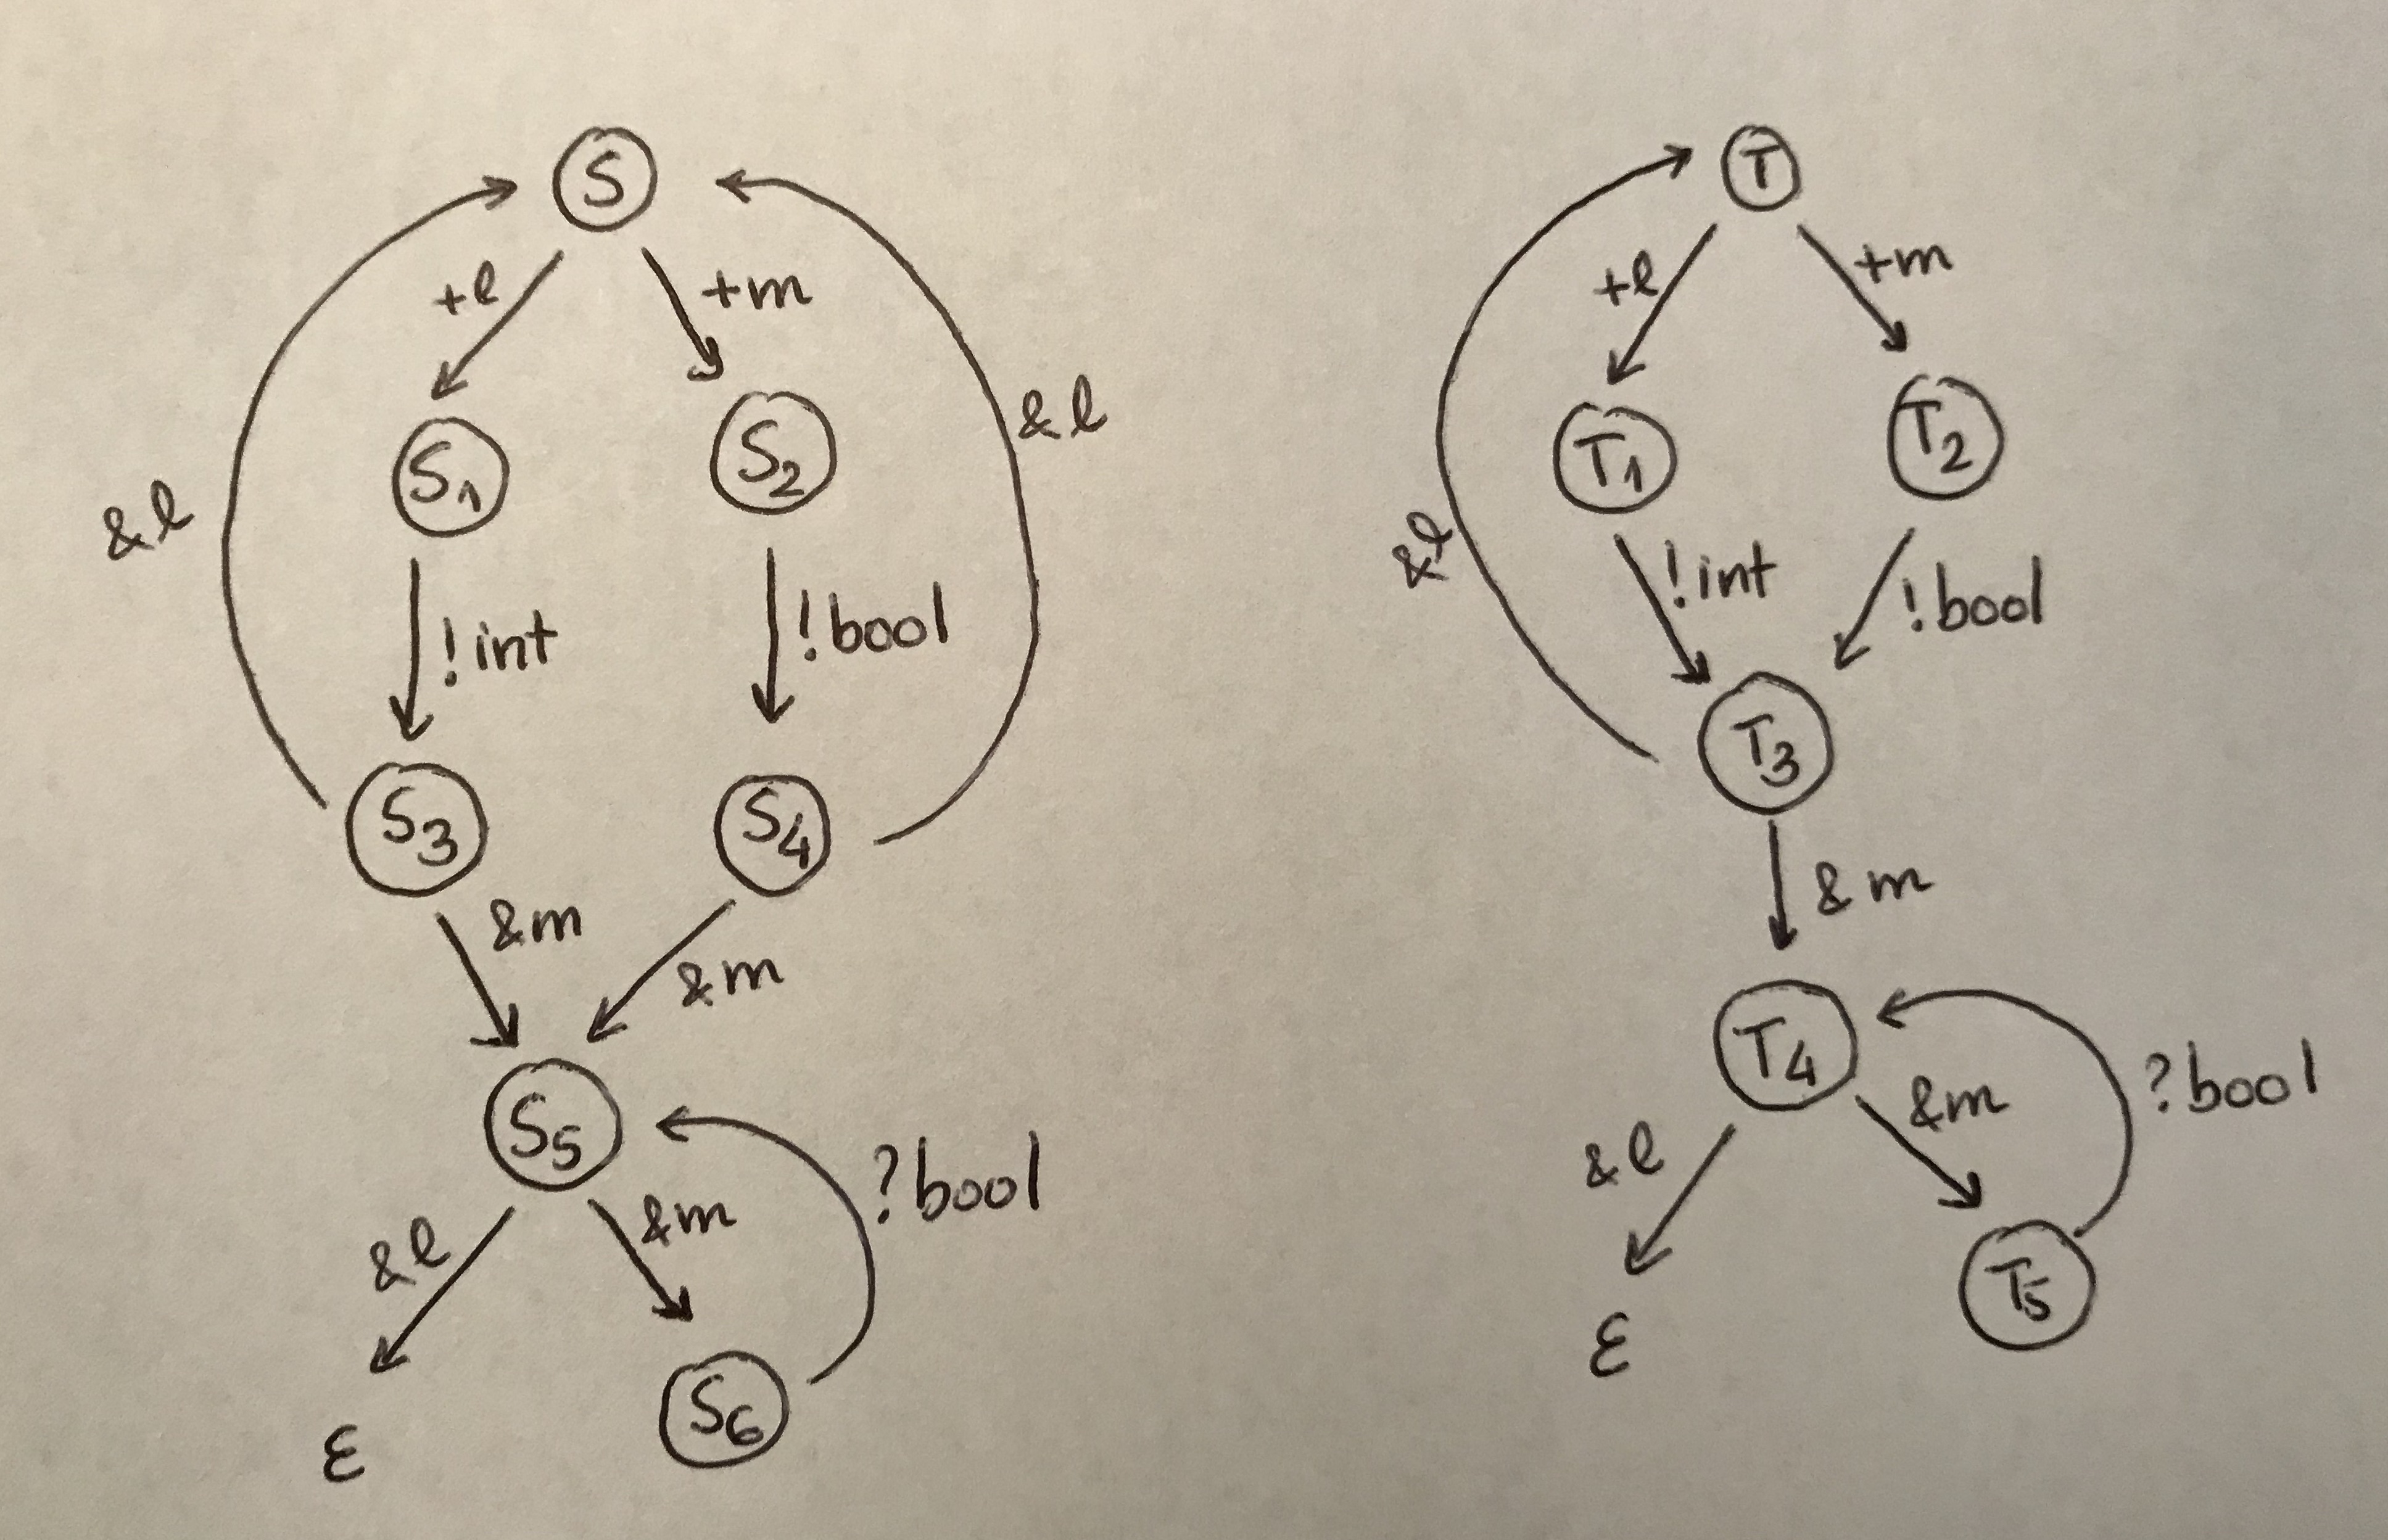
\includegraphics[width=\columnwidth]{PAgraphsST.jpg}
% 		\caption{Process algebra graphs for $S$ and $T$.}
% 			\label{fig:PAgraphsST}
% 	\end{figure}
% 	The algorithm we propose in this work derives the expansion tree for $S\sim T$ as a sequence of nodes. The nodes in this expansion tree can be labeled with a trace of the nodes that lie ahead, based on the syntactical structure of $S$ and $T$. We get the following sequence of labeled nodes in the expansion tree for $S\sim T$:\\\\
% \begin{tikzcd}[cells={nodes={draw=black}}, column sep=large]
%   \enspace (S,T) \enspace \ar[r,"expand"]
% & \enspace  (S_1S_3S_5,T_1T_3), (S_2S_4S_5, T_2T_3) \enspace \ar[r,"expand"]
% & \enspace  (S_3S_5,T_3), (S_4S_5, T_3) \enspace  
% \end{tikzcd} 
% $\xrightarrow{\text{expand}}$\\\\
% \begin{tikzcd}[cells={nodes={draw=black}}, column sep=large]
% & \enspace(SS_5,T),(SS_5,T),(S_5,T_4),(S_5,T_4)  \enspace\ar[r,dashed,"bpa1"]
% &\enspace (S_5,\varepsilon),(S_5,T_4) \enspace 
% \end{tikzcd} 
% $\xrightarrow{\text{expand}}$ \\\\
% \begin{tikzcd}[cells={nodes={draw=black}}, column sep=large]
% &\enspace (S_6S_5,T_5T_4), (\varepsilon,\varepsilon) \enspace \ar[r,dashed,"reflex"] 
% &\enspace (S_6S_5,T_5T_4)\enspace \ar[r,"expand"]
% & \enspace(S_5,T_4)\enspace \ar[r,dashed,"bpa1"]
% &\emptyset\\
% \end{tikzcd}

% 	The process alternates between simplification and expansion operations, denoted by dashed and solid arrows, respectively. Having reached an empty node, we conclude that $S\sim T$.\\\smallskip
	
% 	Now consider the types:
% 	\[ R \triangleq \mu x.\&\{\ell\colon ?\,\boolk;x, m\colon ?\,\intk;x;x \} \text{ and }  U \triangleq \mu x.\&\{\ell\colon ?\,\boolk, m\colon ?\,\intk;x;x\} \enspace .\]
	
% 	$R$ and $U$ are represented as PA graphs as shown in Figure~\ref{fig:PAgraphsRU}.
	
% 	\begin{figure}[h!]
% 	\centering
% 		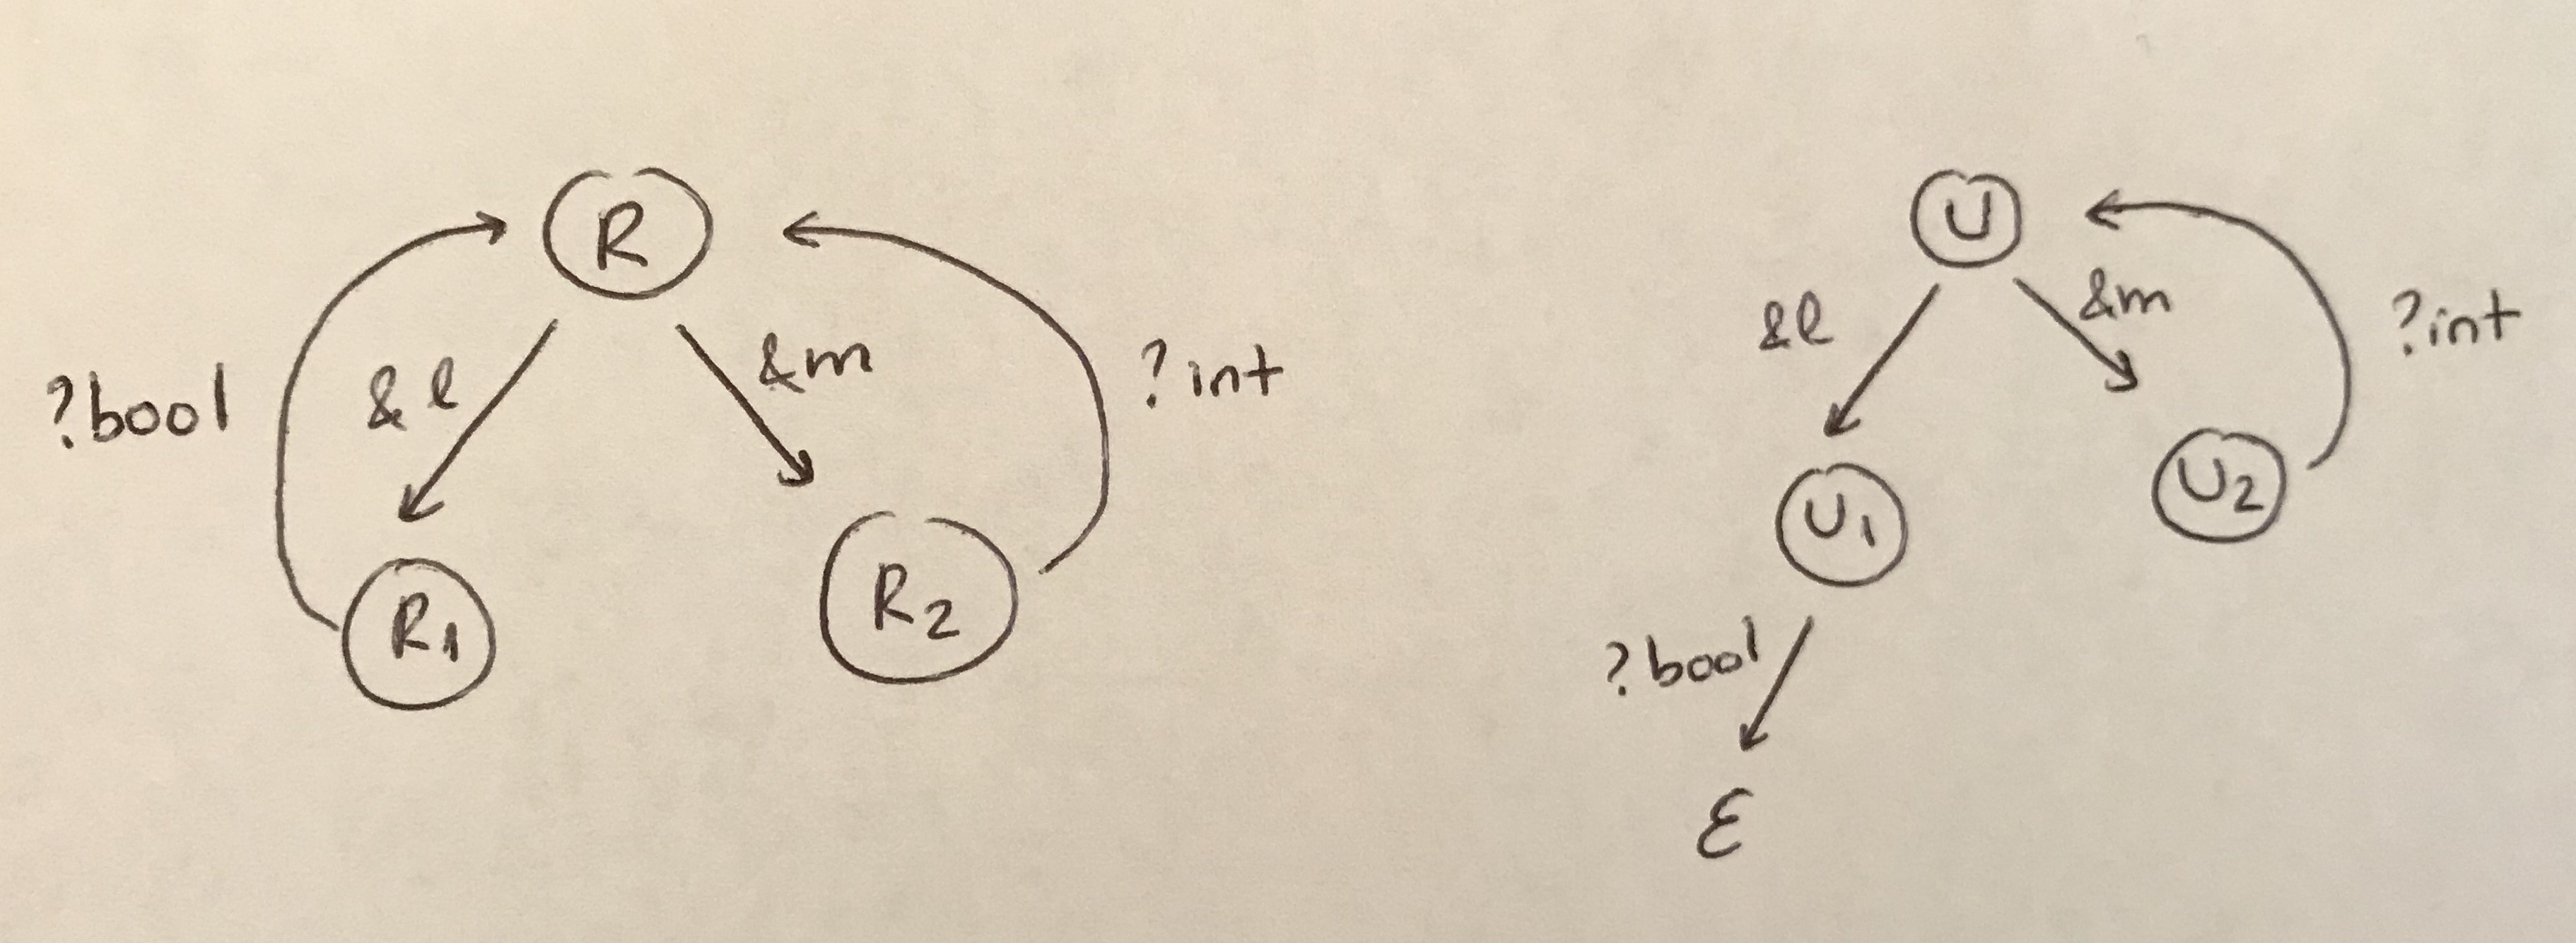
\includegraphics[width=14cm]{PAgraphsRU.jpg}
% 		\caption{Process algebra graphs for $R$ and $U$.}
% 		\label{fig:PAgraphsRU}
% 	\end{figure}
% 	Using the porposed algorithm, we get the following expansion list build upon the syntactical structure of $R$ and $U$ and their representations as PA graphs:\\\\
% \begin{tikzcd}[cells={nodes={draw=black}}, column sep=large]
%   (R,U) \ar[r,"expand"]
% & (R_1 R,U_1), (R_2 R R, U_2 U U) \ar[r,"expand"]
% & (R,\varepsilon), (RR, UU) \ar[r,dashed,"bpa1"] 
% & (R,\varepsilon), (U,\varepsilon) 
% \end{tikzcd} 
% \enspace  $\times$\\\\
% We notice that the last step results from applying BPA1 rule~\cite{janvcar1999techniques} to $(RR,UU)$ knowing that $(R,U)$ is an ancestor node, which leads to the pairs $(R,\varepsilon)$ and $(U,\varepsilon)$. As we then fail to obtain new derived nodes, we decide the type equivalence negatively and conclude that $R\not\sim U$.
% 	\hfill $\triangle$
% \end{example}


%%% Local Variables:
%%% mode: latex
%%% TeX-master: "main"
%%% End:


\end{document}

%%% Local Variables:
%%% mode: latex
%%% TeX-master: t
%%% End:
